\documentclass[border=6pt]{standalone}
\usepackage{amsmath}
\usepackage{amssymb}
\usepackage{tikz}
\usepackage{pgfplots}
\pgfplotsset{compat=1.18}
\usetikzlibrary{arrows.meta,calc,positioning}
\begin{document}
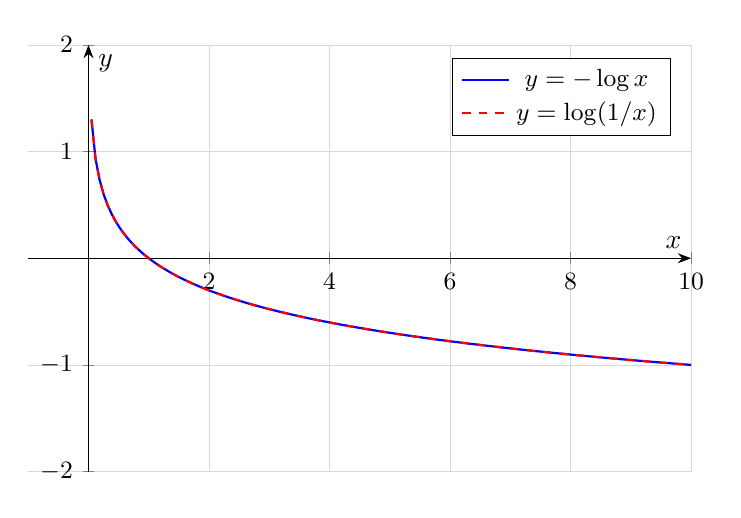
\begin{tikzpicture}
\begin{axis}[
    axis lines = middle,
    xlabel = {$x$}, ylabel = {$y$},
    grid=both,
    grid style={line width=.1pt, draw=gray!30},
    axis line style={-Stealth},
    legend style={font=\small},
    tick label style={font=\small},
    xmin=-1, xmax=10, ymin=-2, ymax=2,
    xtick={0,2,4,6,8,10},
    ytick={-2,-1,0,1,2},
    width=10cm, height=7cm,
    legend pos=north east,
]
\addplot[domain=0.05:10, samples=150, thick, blue] {-(ln(x)/ln(10))};
\addlegendentry{$y=-\log x$}
\addplot[domain=0.05:10, samples=150, thick, red, dashed] {ln(1/x)/ln(10)};
\addlegendentry{$y=\log(1/x)$}
\end{axis}
\end{tikzpicture}
\end{document}
